\cotefile{77}
\scanpage{2}
Formes quadratiques de rg $2$, \deleted{\unsure{à|et}} droites projectives et revêtements quadr.
% archive sheet number: 1
\scanpage{3}
\uline{Digression quadratique}
\margin{cf aussi notes sur $\mathrm{GP}(1)\simeq\mathrm{SO}(3)$ et variantes}

$S$ schéma

$C_1(S)$ catégorie des Modules quadratiques réguliers de rg $2$ $(V,q)$

$C_2(S)$ catégorie des quadruples $(A,V,\xi)$
\[
\text{où }\left\{\begin{aligned}
&A\text{ Algèbre finie étale de rg }2\text{ sur }S\\
&V\quad A\text{-Module inversible}\\
&\text{et }\xi\in\Gamma N_{A/S}(V)^{*}\quad\deleted{\text{section de }N_{A/S}(V)}
\end{aligned}\right.
\]

$C_3(S)$ catégorie des \deleted{triples} \deleted{$(\unsure{D})$} $(\unsure{\mathcal U|U},\deleted{\unsure{S}}T)$, $\mathcal U$ une \deleted{\unsure{forme}} forme de $\mathrm G_m$, et \deleted{\unsure{$S$}}$T$ un $\mathcal U$-torseur

$C_4(S)$ catégorie des couples $(X,\Delta)$, $X$ fibré en droites projectives sur $S$, $\Delta$ un diviseur relatif \inserted{étale} de rang $2$

$C_5(S)$ catégorie des triples $(P,X,D)$, $P$ fibré en \deleted{droites}\inserted{plans} projectifs, $D$ \deleted{droite} ss fibré en droites projectives, $X$ conique lisse de $X$, $D$ et $X$ non tangts. en chaque fibre

% margin note written sideways
\margin{$C_9(S)$ : forme $G$ de $\mathrm{GP}(1)_{/S}$, avec \deleted{\unsure{ss-gpe}} tore maximal $\mathcal U$ de $G$}
% margin note written sideways
\margin{$\unsure{C_{9'}|C'_9}(S)$ forme $G$ de $\mathrm{SL}(2)_S$, avec tore maximal \inserted{$\mathcal U$} de $G$}

$C_6(S)$ catégorie des couples $(E,C)$, $E$ fibré affine de rg $2$, sur $S$, $C\subset E$ conique, projectivement lisse et \deleted{partout} non parabolique en tte fibre.

$C_7(S)$ \deleted{triples}\inserted{quadruples} $(\unsure{\mathcal E|E},Q,\omega,V)$, \inserted{\unsure{où}} $(\mathcal E,Q,\omega)$ une forme \uline{spéciale}-orthogonale de rang $3$, $V$ un sous-\deleted{Module} fibré vect. de rg $2$ \deleted{tel} non isotrope (i.e. telle que $Q|V$ soit régulière)

$C_8(S)$ Catégorie des couples $(M,A)$, $M$ Alg. d'Azumaya de rg $4$ sur $S$, $A$ sous-Algèbre comm. étale de rg $2$.
% archive sheet number: 2
\scanpage{4}
$C_{10}(S)$ Catégorie des torseurs sous $(\mathbb Z/2)_S\mathbin{\cdot}_{1/2}\mathrm G_{m\,S}$.

\deleted{\uline{\illegible{1}}} Toutes ces catégories sont canoniquemt équivalentes...

\deleted{Condition équi} Pour $S'$ sur $S$ fixé (NB $S'=\uline{\operatorname{Spec}}(A)\ldots$) les structures en question forment une \inserted{\unsure{Gr-|cat}} catégorie (clair sur $C_2$ et sur $\unsure{C_3|C_0}$). Si $T$ est un objet de celle-ci ($\unsure{\mathcal U|U}$-torseur), on veut que $T^{\wedge 2}$ est \uline{loc. trivial au sens de Zariski}.
% slanted
\margin{faux, m\textsuperscript{m} sur un corps p.ex. sur $\mathbb R$ la forme quadratique \unsure{$a$|$\alpha$}$(x^2+y^2)$ n'est pas isom. à $xy\ldots$}
 On veut expliciter ce qu'est une trivialisation de $T^{\wedge 2}$. Par la suite exacte de Kummer $0-\mu_2-\mathcal U\xrightarrow{2}\mathcal U\longrightarrow 0$, on voit qu'il revient au $\unsure{=}$ de se donner une restriction du gpe structural à $\mu_2$, ou une orbite \deleted{sous} de $T$ sous $\mu_2$, ou un morphisme de degr $2$ $X\longrightarrow X'$, où $X'$ est un fibré en droites avec diviseur \inserted{relatif} étale $\Delta'$, et une section \deleted{\unsure{de}} de $X'\setminus\Delta'$, $X-X'$ induisant un morphisme \inserted{fini} étale
% slanted
\margin{\uline{NB} L'action de $\mu_2$ sur $(X,\Delta)$ est l'unique action fidèle qui induit l'\uline{identité} sur $\Delta\ldots$ Cf \uline{définition} antérieure d'une cat.\ldots)}
 $X\setminus\Delta\longrightarrow X'\setminus\Delta'$. \unsure{Celà|Cel|Ceci} signifie aussi qu'on a une restriction du Groupe structural au ss-gpe $(\mathbb Z/2)_S\mathbin{\cdot}_{1/2}\mu_{2\,S}\simeq(\mathbb Z/2)_S\times(\mu_2)_S$ agissant sur $\underline O_S\times\underline O_S$ par symétrie et homothéties, Donc la catégorie de ces objets
% slanted
\margin{\uline{NB} $X'=X/\mu_2$ est défini canoniquement, le difficile est de \unsure{m\textsuperscript{e}|mettre} la section de $X'\setminus\Delta'$. \unsure{Chois.|Chos.} $\mathbb Z/2\mathbb Z=\mathbb D_S=\underline O(2)_S$ ($1/2$ \unsure{divisé|disons})}
 s'identifie à la cat. des triples $(A,L,\varepsilon)$, $A$ Algèbre finie étale de rg $2$, sur $S$, $L$ mod. inv. sur $S$, $\varepsilon$ une trivialisation de $L^{\otimes2}$ -- on prend $V=A\otimes_{\underline O_S}L$, d'où $N_{A/\underline O_S}V\simeq L^{\otimes2}$, et on prend $\xi=\varepsilon\ldots$

% archive sheet number: 3
\scanpage{5}
\deleted{$\tau_0\tau_2=\tau_2\tau_0$} \unsure{i.e.}

Donnée (en plus de $X$ fibré en droites projectives) \inserted{d'une Alg. de quatern. $M$} $\Rightarrow C$ assoc. proj.

\diagram{\resizebox{\linewidth}{!}{\begin{tikzcd}[ampersand replacement=\&,row sep=small,column sep=tiny]
{\deleted{\unsure{\exists}}\ \underbrace{\tau_0\ \tau_1\ \tau_2}}\arrow[d,Leftrightarrow]\&{\in\operatorname{Aut}(X)\quad\text{réflexions }(\text{i.e. }\tau_i^2=\mathrm{id},\ \tau_i\ne1\text{ chaque fibre})}\\
{\overbrace{h_0,h_1,h_2}}\arrow[d,Rightarrow]\&{\in\Gamma(C\setminus X)}\\
{L_0,L_1,L_2}\&{\text{orth. (droites des pts fixes des }\tau_0^C,\tau_1^C,\tau_2^C\text{)}}
\end{tikzcd}}}
\margin{\uline{NB} les $\tau_i$ se verraient de façon canonique \deleted{\unsure{en des}} à un signe près en des \deleted{\unsure{élts de}}\inserted{réflexions} \deleted{\unsure{$G$}}$M^*$}

\uline{Hyp}
\[
\left\{\begin{aligned}
&A)\quad\tau_0\tau_2=\tau_2\tau_0.\quad\text{i.e. } A')\ h_0\perp h_2\\
&B)\quad\tau_0\tau_1\ne\tau_1\tau_0,\quad\tau_1\tau_2\ne\tau_2\tau_1\quad\text{sur chaque fibre}\\
&\qquad\text{ou }\beta_{\unsure{3|1|f}}^2\ne1,\ \beta_{\unsure{5|0|s}}^2\ne1\\
&\qquad\text{i.e. } B')\ h_0\not\perp h_1,\quad h_1\not\perp h_2\quad+\quad\text{---}\\
&\qquad(\text{ou }h_0\notin L_1,\ h_1\notin L_2\quad\text{---})
\end{aligned}\right.
\]
% slanted
\margin{ceci, plus $\tau_i^2=\mathrm{id}$ $(i=0,1,\unsure{2|3})$ impliquent que les $\tau_i$ sont des réflexions (ou $\tau_i^2\ne1$ sur chaque fibre)}
% slanted
\margin{ceci implique aussi, déjà, que $h_i\notin X$ sur chaque fibre $(i=0,1,2)$}

\deleted{C) Les $\tau_0,\tau_1,\tau_2$ \unsure{déf.} \unsure{droites} i.e. pts fixes des $\tau_i$ distincts}

\deleted{C) Les $h_0,h_1,h_2$ engendrent le}

\deleted{C') $h_i\notin\Gamma X$ $(i=0,1,2)$ sur tte fibre}

C) $\{h_0,h_1,h_2\}$ engendre tout $C$ en chaque fibre

% slanted
\margin{comment l'exprimer en termes des opérations $\tau_i$ sur \uline{$X$} ?}
($\Longleftrightarrow H_0,H_1,H_2$ indép. en chaque fibre)

D) Considérons la droite \inserted{$H_1\cap H_2$} de $\check{\mathbb P}(M)\supset C\simeq\check{\mathbb P}(\unsure{\gamma M|\mathscr V M})$ formée des pts orth. à $h_1,\deleted{\unsure{h_0}},h_2$ i.e. fixes par $\tau_1,\tau_2$. \deleted{On voit qu'elle ne sont pas tang} \inserted{Les conditions précédentes impliquent qu'en tte fibre,} elle est non contenue dans la quadrique can. de $\check{\mathbb P}(M)$ (définie par le déterminant).

On exige qu'elles \unsure{ne} \unsure{sont|soit} \unsure{pas} tangentes \inserted{en tte fibre}, ce qui signifie aussi que $\beta\deleted{\unsure{=|\ne}}2$ \unsure{sur|inv.}, ou encore que a) Aux pts \inserted{de $S$} de car. $p>0$, \inserted{impaire,} on veut que l'ordre de $\tau_1\tau_2$ soit $\ne p$ (celà suffit \inserted{sur les pts de car. $>0$ \deleted{sont \unsure{d'ordre} \unsure{puisque} \unsure{contr.}} \inserted{\unsure{tous deux|des deux|deux} \unsure{supp.|pts}} \deleted{\unsure{Compte}} \deleted{il faut \unsure{faire}}} car si $\tau_1\tau_2$ d'ordre fini -- sinon on \unsure{cont|contre} aux pts de car. rés. nulle.
% slanted
\margin{il suffit m\textsuperscript{m} pour tte composante irréductible de $S$ contenant un point de car. $p>0$ !}
% archive sheet number: 4
\scanpage{6}
\diagram{\begin{tikzcd}[ampersand replacement=\&,column sep=large,row sep=tiny]
X\arrow[r,leftrightarrow]\&M\arrow[r,leftrightarrow]\&{(X\subset C)}\arrow[d,equal]\\
\&\&{\check{\mathbb P}(\underbrace{\unsure{\gamma|\mathscr V}M}_{V})}
\end{tikzcd}}

\diagram{\resizebox{\linewidth}{!}{\begin{tikzcd}[ampersand replacement=\&,row sep=small,column sep=small,execute at end picture={
\draw ([xshift=-4pt]current bounding box.west |- aa.center) to[out=180,in=90] ([xshift=-9pt]current bounding box.west |- bb.center) to[out=-90,in=10] ([xshift=-14pt]current bounding box.west |- cc.center) to[out=-10,in=90] ([xshift=-9pt]current bounding box.west |- dd.center);
\draw ([xshift=-3pt]current bounding box.west |- cc.center) to[out=180,in=90] ([xshift=-7pt]current bounding box.west |- dd.center) to[out=-90,in=180] ([xshift=-2pt]current bounding box.west |- ee.center);
}]
{\text{réflexions de }X}\arrow[d,leftrightarrow]\\
{\text{réflexions de }C\text{ orthog pour }X}\arrow[d,leftrightarrow]\arrow[r,leftrightarrow]\&{\text{réflexions de }V\text{ orth.}}\\
|[alias=aa]|{\text{pts de }C\setminus X}\arrow[d,leftrightarrow]\\
|[alias=bb]|{\text{droites de }\underset{{}=\gamma M}{V}\text{ non \uline{isotropes}}}\arrow[d,leftrightarrow]\&{M^*,\quad\operatorname{Tr}u-}\\
|[alias=cc]|{\text{divis. }\inserted{\text{étales}}\text{ de degr }2\text{ sur }X}\arrow[d,leftrightarrow]\&\deleted{\unsure{\simeq}}\\
|[alias=dd]|{\text{\deleted{droites} droites de }C\text{ non tgtes à }X}\arrow[d,leftrightarrow]\\
{\text{plans de }V\ (\text{ou de }\gamma M)\text{ non tangents au cône }q=0}\arrow[d,leftrightarrow]\\
|[alias=ee]|{\text{Sous-Algèbres étales de rg }2\text{ de }M}\arrow[d,leftrightarrow]\\
{\text{Elémts }\sigma\text{ de }M\ (\text{tels que }\deleted{\unsure{\sigma}}\inserted{\text{qui sont des \uline{réflexions}, i.e.)}}\deleted{\text{tels}}}
\end{tikzcd}}}
\margin{car. $\ne2$ sinon il faut en enlever quelquechose}
\margin{car $\ne2$}
\[
\begin{aligned}
&\sigma^2=1,\quad \sigma\ne\pm1\text{ chaque fibre (condition}\\
&\deleted{\text{qui suppose }2\unsure{\text{ inv.}}\ \text{car.}\ne2}\\
&\text{équiv. pour }2\text{ régulier sur}\\
&\boxed{\det\sigma=-1}\,)
\end{aligned}
\]

L'action (via transport de structure) de la réflection $\tau$ sur $M$, en termes de $\sigma$, est $u\longmapsto\sigma u\sigma^{-1}$ -- mais ce \uline{n'est pas} une réflection de $M$ ! (val. propres $1,-1$ avec mult. $2$ l'une et l'autre) Pour avoir une réflexion, il faut \deleted{\unsure{conjuguer}}\inserted{composer} avec $u\longmapsto u^*=\operatorname{Tr}u.1-u$ !!!

On a
\[
\boxed{\widetilde\sigma(u)=\sigma u^*\sigma=(\sigma u\sigma)^*=u-\operatorname{Tr}(u.\sigma)\sigma}
\]
% archive sheet number: 5
\scanpage{7}
\margin{(\unsure{130|136|13 p})}
Formes quadratiques inv. et quasi-inv. sur $D_\infty,D_n$
\mspage{\unsure{1}}
% archive sheet number: 6
\scanpage{8}
Formes quadratiques quasi-invariantes sous le groupe diédral.

\uline{Cas I} $\alpha\ne\pm2$ fibre par fibre \inserted{($\alpha^2-4$ inv.)}, de sorte que la repr. \deleted{affine}\inserted{projective} (ou affine) envisagée de $\mathbb D_\infty=\operatorname{Aut}(\unsure{\underline\Phi|\Phi|\Omega}\deleted{\unsure{\infty}})$ se restreint en une représentation vectorielle où
\[
\begin{aligned}
&\sigma(x,y)=(y,x)\qquad \sigma'(x,y)=(\unsure{\zeta|\xi}y,\zeta^{-1}x)\\
&u(x,y)=(\zeta x,\zeta^{-1}y)
\end{aligned}\tag*{(1)}
\]
La décomposition $E=D_1\oplus D_2\oplus D_0$ (correspondant aux val. propres $\zeta,\zeta^{-1}$ de $u$\unsure{$\}$|,}, $\zeta\ne\zeta^{-1}\ne1$ fibre par fibre) définit une décomposition analogue de
\[
\operatorname{Sym}^{2}(\check E)\simeq
\check D_1^{\otimes2}\oplus\check D_2^{\otimes2}\oplus\check D_0^{\otimes2}
\oplus\check D_1\otimes\check D_2\oplus\check D_1\otimes\check D_0+
\check D_{\unsure{1|2}}\otimes\check D_0
\tag*{(2)}
\]
correspondant aux valeurs propres
\[
\zeta^{-2},\ \zeta^{\unsure{+2|2|-2}},\ 1,\ 1,\ \zeta^{-1},\ \zeta^{+2}
\tag*{(3)}
\]
de $u$.

Supposons d'abord les \inserted{\unsure{5|6}} val. propres $1,\zeta,\zeta^{-1},\zeta^{2},\zeta^{-2}$ distinctes deux à deux fibre par fibre (ce qui signifie $\zeta^3\ne1,\zeta^4\ne1$ fibre par fibre, en plus de $\zeta\ne\pm1$ \inserted{fibre par fibre i.e. $(\zeta^2-1)$ inv.,} exprimant $\alpha\ne\pm2$ fibre par fibre...)

Alors les droites propres pour $u$ sont \deleted{celles qui} d'une part $\check D_1^{\otimes2},\check D_2^{\otimes2},\check D_1\otimes\check D_0,\check D_2\otimes\check D_0$, d'autre part les droites contenues \inserted{\unsure{loc.|les|(ens)}} dans $\check D_0^{\otimes2}\oplus(\check D_1\otimes\check D_2)$.

Or les $4$ droites précédentes sont non inv. par $\sigma$ (qui échange $\check D_1$ et $\check D_2$, donc $\check D_1^{\otimes2}$ et $\check D_2^{\otimes2}$, $\check D_1\otimes\check D_0$ et $\check D_2\otimes\check D_0$), d'autre part $\sigma$ opère trivialemt dans $\check D_0^{\otimes2}\oplus(\check D_1\otimes\check D_2)$. Donc on trouve, \deleted{les dr}\inserted{comme}
% archive sheet number: 7
\scanpage{9}
seules droites invariantes \inserted{\unsure{pour|par} $\mathbb D_\infty$} de $\operatorname{Sym}^2(\check E)$, \deleted{les} celles qui sont \unsure{formées|fournies} de formes quadratiques \uline{invariantes}.

Si on permet \deleted{que} ${\unsure{\zeta|\xi}}^3=1$ sur certaines fibres, \margin{i.e. $\alpha=-1$ sur certaines fibres} \deleted{alors on} mais pas $\zeta^4=1$, alors on trouve que les droites inv. dans $\operatorname{Sym}^2(\check E)$ pour $u$ sont contenues \inserted{loc.} dans $V=\check D_1^{\otimes2}\unsure{\oplus}\check D_2$ ou $\unsure{W|V}=\check D_2^{\otimes2}\oplus\check D_1$ ou $\check D_0^{\otimes2}\oplus\check D_1\otimes\check D_2$, or $\sigma$ échange $V$ et $W$, donc il n'y a pas de droite inv. par $\Phi$ ni dans $V$, ni dans $W$, et on \deleted{\unsure{est dans les}}\inserted{obtient la} $=$ conclusion.

Mais si on permet $\zeta^4=1$ sur certaines fibres, que se passe-t-il ? Supposons donc carrément \deleted{$\zeta^4$}
\[
\zeta^4=1\qquad\text{i.e.}\qquad\zeta^2=-1,\ \text{ou encore }\alpha=0
\tag*{(4)}
\]
(cas du carré) -- car (4) s'écrit
\[
(\zeta^2-1)(\zeta^2+1)=0
\]
et comme par hyp. $\zeta^2-1$ est inv, celà donne $\zeta^2+1=0$ i.e. $\zeta+\zeta^{-1}=0$ i.e. $\alpha=0\ldots$

Alors les valeurs propres distinctes parmi (3) sont $\zeta^2=\zeta^{-2}=-1,\ 1,\ \zeta,\zeta^{-1}$, correspondant aux sous-espaces propres $\check D_1^{\otimes2}\oplus\check D_2^{\otimes2},\check D_0^{\otimes2}\oplus(D_1\otimes D_2),\check D_1,\check D_2$. Les droites propres
% archive sheet number: 8
\scanpage{10}
sous $u$ sont celles contenues dans un de ces sous-espaces. Si on veut qu'elles soient aussi inv. sous $\sigma$, il ne reste plus que les droites \unsure{des|dans} les deux premiers sous-espaces. Or on est en car. $\ne2$ (car ${\unsure{\zeta|\xi}}^2=-1$, mais $\zeta^2\ne+1$ fibre par fibre) et $\sigma$ opère sur $\check D_1^{\otimes2}\oplus\check D_2^{\otimes2}$ en permutant $\check D_1^{\otimes2}$ et $\check D_2^{\otimes2}\ldots$ Cela fait donc $2$ droites propres exactement de l'espace qu'ils engendrent, correspondant aux val. propres $+1$ et $-1$ resp. pour $\sigma$, les val. propres pour $u$ étant $-1,-1$, celles pour $\sigma'\inserted{=u\sigma}$ \deleted{étant} donc $-1,1$.

Si on \deleted{\unsure{expr|appr}} récrit le cadre en coordonnées $(x,y)$ avec sommets $(\pm1,\pm1)$ \deleted{\unsure{du carré|de côtés}} se suivant dans l'ordre
\[
(1,1),(-1,1),(-1,-1),(1,-1)
\]
\figure{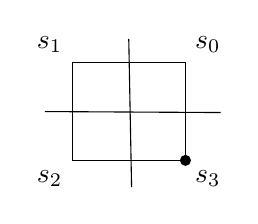
\begin{tikzpicture}[x=.72cm,y=.62cm]
\draw (-1,1)--(1,1)--(1,-1)--(-1,-1)--cycle;
\draw (-1.48,0)--(1.62,-.02); \draw (0,1.49)--(.05,-1.55);
\fill (1,-1) circle (2pt);
\node[above left] at (-1,1) {$s_1$}; \node[above right] at (1,1) {$s_0$};
\node[below left] at (-1,-1) {$s_2$}; \node[below right] at (1,-1) {$s_3$};
\end{tikzpicture}}
\margin{\uline{NB} car $\ne2$}
Les formes quadratiques en $(x,y,z)$ correspondantes sont $x^2-y^2\inserted{=(x-y)(x+y)}$ et $xy$ (\uline{NB} $\sigma(x,y)=(y,x)$ $\sigma'(x,y)=(-x,y)$).

\deleted{\uline{elles sont toutes deux \inserted{non} dégénérées}.} [La première prend la valeur constante \deleted{\unsure{$4$|$\ne$}}$0$ sur les sommets du carré, la seconde prend la valeur $+1$ sur \inserted{un couple de} deux sommets opposés, la valeur $-1$ sur le couple des deux autres sommets... ] Seule la première définit une conique inv. passant par les sommets du carré, savoir la
% archive sheet number: 9
\scanpage{11}
conique $x^2-y^2=0$, mais celle-ci a l'origine comme pt singulier. C'est une réunion des deux droites diagonales.

\margin{bref !}
On voit \uline{donc} que si ${\unsure{\zeta|\xi}}^{4}-1$ est inv. i.e. \deleted{\unsure{$\zeta$|$4$}}$(\alpha^2-4)$ inv., alors \deleted{il y a ex} une forme quadratique sur $E$ quasi-invariante par $\Phi$ \uline{et non dég.} sur chaque fibre est en fait invariante par $\Phi$, et c'est une combinaison linéaire des formes $z^2$ et $xy$ (avec les coordonnées choisies\unsure{\}|)}, \deleted{qui} où on a dû d'abord faire un changt de base quadratique vers
\[
S'=\operatorname{Spec}\underline O_S[T]/(T^2-\alpha T+1)\quad\ldots\,)
\]
\[
Q(x,y,z)=az^2+bxy\tag*{(5)}
\]
de \deleted{déterminant} matrice
\[
\begin{pmatrix}0&b&0\\b&0&0\\0&0&2a\end{pmatrix}
\]
de déterminant
\[
\delta(Q)=2ab^2\tag*{(6)}
\]
donc de déterminant divisé
\[
\delta'(Q)=ab^2\tag*{(7)}
\]
\unsure{(qui|Qui} est \deleted{\unsure{inversible}}\inserted{inv.} \unsure{sss|ssi} $a,b$ le sont. La condition que $Q$ s'annule sur les sommets de $P$ s'écrit alors
\[
a+b=0\tag*{(8)}
\]
donc \deleted{\unsure{les}} $\exists!$ \deleted{\unsure{f.}} \unsure{côniques|cônique} circonscrites à $P$ invariantes sous $\mathbb D_\infty$, \deleted{sont} d'équation
\[
z^2-xy=0\tag*{(9)}
\]
Ou encore, en coordonnées affines, $\exists!$
% archive sheet number: 10
\scanpage{12}
\inserted{à scalaire près} \deleted{fonction quadratique sur}\inserted{poly. de degré $\leq2$} $\unsure{V|F}$ invariante par $\mathbb D_\infty$ et \deleted{\unsure{non-dégén}}nulle sur les sommets du polygône $P$, savoir
\[
xy-1
\]
[ou encore, $\exists!$ forme quadratique sur $V$ invariante par $\mathbb D_\infty$ égale à $1$ sur les sommets du polygône $P$, savoir $xy\ldots$ ].

\uline{NB} Il y a ``en général'' une et une seule cônique qui passe par cinq points. (\uline{NB} cinq équations lin. \unsure{strictes|scalaires|homogènes} sur $6$ coeff. homogènes...), donc \deleted{on} s'attend à ce \deleted{que}, lorsque $P$ a au moins cinq pts fibre par fibre (i.e. $\alpha\ne0,-1$ fibre par fibre pour exclure triangles et carrés, donc au total
\[
\alpha(\alpha^2-4)(\alpha+1)\quad\text{inversible}
\]
qu'il existe \deleted{\unsure{$\exists$}}\inserted{une unique} conique qui passe par les sommets de $P$. Écrivant la cônique sous forme non homogène comme
\[
Q(x,y)=ax^2+\deleted{\unsure{2}}bxy+cy^2+ux+vy+\lambda
\]
et prenons pour $(x,y)$ les cinq points $({\unsure{\zeta|\xi}}^i,\zeta^{-i})$, $-2\leq i\leq+2$, on trouve
% archive sheet number: 11
\scanpage{13}
les conditions sur $a,b,c,u,v,\lambda$ s'expriment par un syst. de $5$ équ. lin., de matrice
\[
\begin{pmatrix}
1&1&1&1&1&1\\
{\unsure{\zeta|\xi}}^2&1&\zeta^{-2}&\zeta&\zeta^{-1}&1\\
\zeta^{-2}&1&\zeta^2&\zeta^{-1}&\zeta&1\\
\zeta^4&1&\zeta^{-4}&\zeta^2&\zeta^{-2}&1\\
\zeta^{-4}&1&\zeta^4&\zeta^{-2}&\zeta^2&1
\end{pmatrix}
\]
et il faut vérifier si \deleted{un des mineurs} cette matrice \inserted{$5\times6$} est bien de rang $5$ fibre par fibre, ce qui \unsure{ient|est|revient|équivaut} (vu qu'il y a deux colonnes identiques formées de $1$) que le déterminant \deleted{\unsure{de la matr}}
\[
\det\begin{pmatrix}
1&1&1&1&1\\
\zeta^2&\zeta^{-2}&\zeta&\zeta^{-1}&1\\
\zeta^{-2}&\zeta^2&\zeta^{-1}&\zeta&1\\
\zeta^4&\zeta^{-4}&\zeta^2&\zeta^{-2}&1\\
\zeta^{-4}&\zeta^4&\zeta^{-2}&\zeta^2&1
\end{pmatrix}\quad\deleted{\unsure{6}}=\Delta(\zeta)
\]
\margin{où $\Delta\in\mathbb Z[T,\unsure{T^{-1}}]$}
% slanted
\margin{renverser l'ordre des colonnes, pour avoir matrice symétrique}
est inversible. De la façon dont on a obtenu ce déterminant, il \deleted{semble} est clair qu'il est nul si \deleted{\unsure{$\zeta^2=1$}} si $\zeta^3=1$, ou $\zeta^4=1$, i.e. si \inserted{$\zeta$ est une des six racines (\unsure{ttes|lettres} simples, sur $\mathbb Q$) du poly}
\[
\frac{(\zeta^4-1)(\zeta^3-1)}{\zeta-1}\ \in\mathbb Z[\zeta]
\]
\deleted{et \unsure{en pr|$\equiv$ par} $(\zeta^2+1)($}
On trouve que $\Delta(T)$ est divisible par
\[
\frac{(\zeta^4-1)(\zeta^3-1)}{\zeta-1}
=(\zeta^2+1)(\zeta^2-1)(1+\zeta+\zeta^2),\quad\text{et }=\text{ par}
\]
\[
(\zeta^2+1)(\zeta^2-1)^2(1+\zeta+\zeta^2)=\alpha(\alpha^2-4)(\alpha+1)
\]
\margin{Étudier la nullité du dit déterminant \unsure{!|?}}
% archive sheet number: 12
\scanpage{14}
\illegible{2}\unsure{toute} \inserted{fonction pol. de \unsure{degré} \unsure{\illegible{1}|$\leq2$}} $q$ qui s'annu\unsure{le} sur cinq sommets consécutifs s'annule sur tous les sommets (si $\alpha(\alpha+1)$ inversible) et est en fait un multiple de la forme \deleted{quadratiq} invariante principale.

Sur l'espace des translations, la forme quad. principale est
\[
\deleted{\unsure{q_0(x,y)|q(x,y)}}\quad q_{\deleted{\unsure{0}}\unsure{0|\Phi}}(x,y)=x^2+y^2-\alpha xy
\tag*{(3)}
\]
\deleted{qui est dég.} dont le discriminant est
\[
\delta_0=\alpha^2-4=(\alpha-2)(\alpha+2)\tag*{(4)}
\]
inv. sss $\alpha\ne\unsure{\pm|+}2\deleted{\unsure{0}}$ fibre par fibre i.e. sss on est dans cas I.

Quant à $q_0$ elle-même, s'écrit comme forme en $3$ variables $x,y,z$
\[
q_{\unsure{0|\Phi}}(x,y,z)=x^2+y^2\deleted{\unsure{xy}}+0z^2-yz-\unsure{z}x-\alpha xy
\tag*{(2 bis)}
\]
de matrice adjointe
\[
\begin{pmatrix}2&-\alpha&-1\\-\alpha&2&-1\\-1&-1&0\end{pmatrix}
\tag*{(5)}
\]
de discriminant
\[
\delta=\deleted{\unsure{4a+}}-2\alpha\deleted{\unsure{+}}\unsure{-|+}2-2=-2(\alpha+2)
\tag*{(6)}
\]
de discriminant divisé
\[
\delta'=-(\alpha+2)\tag*{(6$'$)}
\]
qui est nul sss $\alpha=-2$, inv. sss $\alpha\ne-\unsure{2|1}$ sur chaque fibre (i.e. si on n'est pas dans cas $\overline{\underline{\mathrm{III}}}$ sur aucune fibre...)
% archive sheet number: 13
\scanpage{15}
Les deux pts isotropes (confondus \deleted{\unsure{sur}} en \unsure{la|chaque} fibre en un $s$ sss $\alpha_s=\deleted{\unsure{+}}-2\ldots$) correspondent aux \deleted{solutions} directions de pente $\unsure{\zeta|\xi}=y/x$ satisfaisant
\[
\zeta^2-\alpha\zeta+1=0\qquad\text{i.e.}\qquad\zeta+\zeta^{-1}=\alpha
\tag*{(7)}
\]
Étudions la situation où on se donne (en plus du polygône épinglé) une telle direction isotrope -- ici le \deleted{schéma} ``module'' est donc \inserted{la section inversible} $\zeta$, plus fin que $\alpha$ [et pour les \deleted{\unsure{ép}} ``$n$-polygônes'' on aura $\Phi_n(\zeta)=0$ \margin{pol. cyclotomique} $+$ condition de caractéristique...] Donc la forme quadratique $q_0$ s'écrit
\[
q_0(x,y)=(x\unsure{-}\zeta y)(x-\zeta^{-1}y)
\tag*{(8)}
\]
et $q(x,y,z)$ s'écrit
\[
q(x,y,z)=(x-\zeta y)(x-\zeta^{-1}y)-(x+y)z
\tag*{(9)}
\]
Utilisons \deleted{\unsure{$\zeta$}} la \deleted{droite du}\inserted{droite $D_\zeta$ de pente $\zeta$ et} le pt isotrope $d_\zeta\in C$ \deleted{de pent\unsure{e} $\zeta$}\inserted{correspondant} pour identifier la cônique $C$ : $q(x,y,z)=0$ à $\mathbb P(E/D_\zeta)$ -- on trouve

\figure{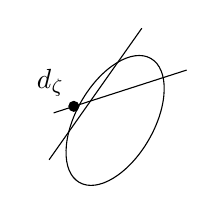
\begin{tikzpicture}[x=.64cm,y=.64cm]
\draw[rotate around={-30:(0,0)}] (0,0) ellipse (.77 and 1.42);
\draw (-1.31,-.78)--(.53,1.83);
\draw (-1.22,.15)--(1.42,1.00);
\fill (-.82,.28) circle (2pt) node[above left] {$d_\zeta$};
\end{tikzpicture}}
Un \unsure{répère|repère} projectif de $\mathbb P(E/D_\zeta$ \unsure{grace|grâce} aux trois plans suivants contenant $D_\zeta$ i.e. aux droites projectives de $\check{\mathbb P}(E)$ contenant $d_\zeta$

\unsure{0)|a)|$\circ$)} \deleted{le plan qui \unsure{correspond}}\inserted{celui qui correspond} la droite tangente à $d_\zeta$ à $C$
% archive sheet number: 14
\scanpage{16}
\[
\left\{\begin{aligned}
f_1&=(1,\unsure{\zeta|\xi},0)=e_1+\zeta e_2\\
f_2&=(1,0,1-\zeta)=e_1+(1-\zeta)\deleted{\unsure{f_3}}e_3
\deleted{=\underbrace{(0,\unsure{\zeta},\unsure{\zeta-1})}_{\text{vecteur directeur de la }2^{\mathrm e}\text{ droite isotrope}}=e_2+(\zeta-1)e_3}\\
f_3&=(0,0,1)=e_3
\end{aligned}\right.
\]
\figure{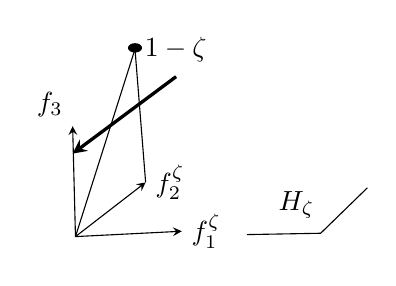
\begin{tikzpicture}[x=.9cm,y=.85cm,>=stealth]
\draw[->] (0,0)--(1.5,.08) node[right] {$f_1^\zeta$};
\draw[->] (0,0)--(.99,.81) node[right] {$f_2^\zeta$};
\draw[->] (0,0)--(-.04,1.65) node[above left] {$f_3$};
\fill (.84,2.82) ellipse (.10 and .07);
\draw (.99,.81)--(.84,2.8) node[right] {\unsure{$1-\zeta$}};
\draw (0,0)--(.84,2.8);
\draw[->,very thick] (1.42,2.39)--(-.04,1.24);
\draw (2.42,.03)--(3.46,.05)--(4.12,.73);
\node at (3.12,.47) {$H_\zeta$};
\end{tikzpicture}}

\uline{NB}
\[
\begin{aligned}
e_1&=f_2-(1-\zeta)f_3=f_2+(\zeta-1)f_3\\
e_2&=\zeta^{-1}(f_1-e_1)=\zeta^{-1}f_1-\zeta^{-1}f_2+(1-\zeta^{-1})f_3\\
e_3&=f_2\\
&\deleted{\unsure{f_2}=\zeta^{-1}f_1\unsure{-}\zeta^{-1}f_2+(1-\zeta^{-1})f_3}
\end{aligned}
\]
Le plan \inserted{$(e_1,e_2)$ est \unsure{insécable|invariable|invariant} !} engendré par $(f_1,e_1)$ (qui correspond à la droite isotrope $D_{\zeta^{-1}}=D'_\zeta\ldots$), qui correspond dans le plan $(f_2,f_3)$ -- (si $\zeta-1$ inv.) à la droite de pente (p.r. à $f_3,f_2$) $\dfrac{1}{\zeta-1}$

\medskip
\deleted{Donnée du Polygone épinglé \inserted{\unsure{pointé|par $\infty$|par $D_\zeta$}} de type $\ne\mathrm{III}$ \deleted{équivaut}\inserted{\unsure{i.e. est équiv|i.e. est ép|i.e. réguliers}} $+$ droite isotrope $\Longleftrightarrow$ donnée de $\zeta\in\Gamma(S,\underline O_S)^*$ $\Longleftrightarrow$ ce qui suit :}

\deleted{1°) fibré \deleted{en droites affines \unsure{$F$} sur $S$ i.e. \unsure{torseur sous|disons un|torseurs sous}} fibré vectoriel \inserted{de rang $1$} \deleted{inv. \unsure{$F$} i.e. est en lien \unsure{$V$|via}}\inserted{$F$} lié par un $L$}

\[
\deleted{0-L-F-\underline O_S\longrightarrow0}
\]
\deleted{2°) Une section de $\mathbb P(F)$ i.e. un Module inv. $L'$ et un hom}
\[
\deleted{F\longrightarrow L'}
\]
Avec ceci, on construit le schéma en groupes
% archive sheet number: 15
\scanpage{17}
\deleted{des autom. de $P$ qui invarient le diviseur \deleted{\unsure{sections|section}} relatif de degré $2$ qui est défini par les $2$ sections de $P$, \uline{et} induisent l'identité dessus -- qui est un schém. en groupes $G$ lisse sur $S$, de dim relative $1$, dont la comp. \deleted{connexe}\inserted{neutre} $G^0$ est commutative}

\deleted{3°)}
% archive sheet number: 16
